\documentclass[aspectratio=169]{beamer}
%\documentclass[aspectratio=169,handout]{beamer}

\usetheme[hidefootline,altlogo=images/ssl-logo_text.png,sidebarwidth=1.9cm]{Oxford}
\usepackage{subcaption}
\usepackage{listings}
\lstset{escapeinside={<@}{@>}}

% TODO: factor into beamer-oxford template
\setbeamertemplate{footline}{}
\setbeamertemplate{page number in head/foot}[framenumber]
\setbeamertemplate{navigation symbols}{\footnotesize\usebeamertemplate{page number in head/foot}\vspace{0.2em}}
\addtocounter{framenumber}{-1}

\begin{document}

\bgroup
\let\oldfootnoterule\footnoterule
\setbeamerfont{footnote}{size=\tiny}

\title[Spoofing Earth Observation Satellites through Radio Overshadowing]{Firefly: Spoofing Earth Observation Satellites through Radio Overshadowing}
\author[Edd Salkield]{
  \emph{Edd Salkield}
  \inst{1}
  \and
  Joshua Smailes
  \inst{1}
  \and
  Sebastian Köhler
  \inst{1}
  \and
  Simon Birnbach
  \inst{1}
  \and
  Richard Baker
  \inst{1}
  \and
  Martin Strohmeier
  \inst{2}
  \and
  Ivan Martinovic
  \inst{1}
}
\institute[--~~Systems Security Lab]{
  \inst{1} Systems Security Lab, University of Oxford \and %
  \inst{2} Cyber-Defence Campus, armasuisse Science + Technology
}
\date{NDSS SpaceSec 2023}

\makeoxfordtitle

\note{
Although satellite data is becoming increasingly important, many satellites don't use cryptography to authenticate the downlink, which opens the door for spoofing attacks.
My name's Edd Salkield, and I'm from the Systems Security Lab at the University of Oxford.
I'm presenting Firefly, an analysis of the vulnerability and effects of spoofing attacks against current Earth observation satellite systems.
In particular, we'll consider the effects of a motivated, modern adversary against NASSA's real-time forest fire API.

The current situation in space is that...
}

\section{Motivation}
\subsection{Challenges}

\def\footnoterule{\only<6->\oldfootnoterule}
\begin{frame}
  \frametitle{Challenges of unauthenticated satellites}
  \begin{itemize}[<+->]
    \item Many current satellites do not encrypt the downlink, due to:
    \begin{itemize}[<+->]
      \item Increased power budget, mission complexity, and cost
      \item Legacy systems backwards compatibility
      \item Open access data
    \end{itemize}
    
    \item Other satellites are decryptable, due to:
    \begin{itemize}[<+->]
      \item Insecure cryptosystems~\footnote<6->{COMS-1 uses single DES \url{https://vksdr.com/lrit-key-dec/}}
      \item Leaked keys~\footnote<7->{GK-2A keys leaked in source code \url{https://vksdr.com/xrit-rx/}}
    \end{itemize}
  \end{itemize}
\end{frame}

\begin{frame}
  \frametitle{Challenges of unauthenticated satellites}
  \framesubtitle{Insecure Earth Observation Satellites}

  Satellites with insecure downlinks include:

  \begin{itemize}
    \item \textbf{Fire detection and management}, e.g., Terra, Aqua
    \pause
    \item Geospatial intelligence, e.g., Landsat-7..9
    \item Weather monitoring, e.g., GOES-14..17, FengYun series
    \item Infrared sensing, e.g., Metop-A,B
    \item Climate monitoring, e.g., Suomi-NPP
  \end{itemize}
\end{frame}

\subsection{Implications}

\def\footnoterule{\only<3->\oldfootnoterule}
\begin{frame}
  \frametitle{Implications}
  \framesubtitle{Data secrecy}

  \begin{center}
    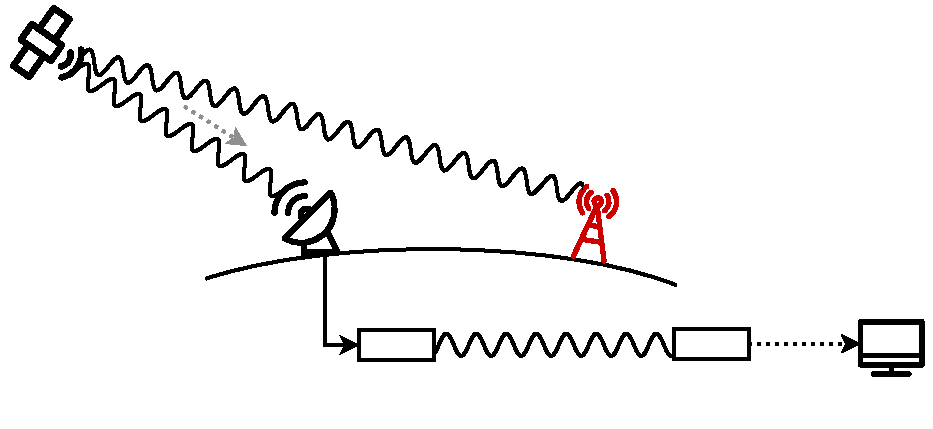
\includegraphics[width=0.7\textwidth]{images/eavesdropping_illustration.pdf}
  \end{center}

  \pause
  \vspace{-0.7cm}

  Using an SDR and open source software, attackers can:
  \pause
  \begin{itemize}[<+->]
    \item Read confidential maritime data\footnote<3->[1]{Pavur et al. (2020) ``\textit{A Tale of Sea and Sky on the Security of Maritime VSAT Communications}''} and internet traffic\footnote<3->[2]{Pavur et al. (2019) ``\textit{Secrets in the Sky: On Privacy and Infrastructure Security in DVB-S Satellite Broadband}''}
    \item Eavesdrop on Iridium traffic and calls~\footnote<4->[3]{muccc ``\textit{Iridium Toolkit}'' \url{https://github.com/muccc/iridium-toolkit}}
  \end{itemize}
\end{frame}

\def\footnoterule{\only<5->\oldfootnoterule}
\begin{frame}
  \frametitle{Implications}
  \framesubtitle{Data authenticity and integrity}

  \vspace{-0.4cm}
  \begin{center}
    \includegraphics<1|handout:0>[width=0.5\textwidth]{images/overshadow_illustration_1.pdf}%
    \includegraphics<2|handout:0>[width=0.5\textwidth]{images/overshadow_illustration_2.pdf}%
    \includegraphics<3->[width=0.5\textwidth]{images/overshadow_illustration_3.pdf}%
  \end{center}

  \pause[4]
  \vspace{-0.5cm}
  Spoofing attacks have been shown against:

  \pause
  \begin{itemize}[<+->]
    \item GNSS to manipulate calculated location\footnote<5->[1]{Motallebighomi et. al. (2022) ``\textit{Cryptography Is Not Enough: Relay Attacks on Authenticated GNSS Signals}''}
    \item Uplinks for satellite hijacking\footnote<6->[2]{``\textit{2011 REPORT TO CONGRESS of the U.S.-CHINA ECONOMIC AND SECURITY REVIEW COMMISSION}'' p.223--224} or broadcast intrusion\footnote<6->[3]{Broadcasting (1986) ``\textit{`Captain Midnight' unmasked}''}
  \end{itemize}

  \pause[\thebeamerpauses]
  No work considers spoofing Earth Observation satellites

  \pause
  \textbf{RQ}: What can the attacker achieve by exploiting the unauthenticated channel of these specific systems?
\end{frame}

\subsection{Threat model}
\begin{frame}
  \frametitle{Threat model}

  \begin{center}
    \includegraphics<1|handout:0>[width=0.7\textwidth]{images/attack_illustration_1.pdf}%
    \includegraphics<2|handout:0>[width=0.7\textwidth]{images/attack_illustration_2.pdf}%
    \includegraphics<3->[width=0.7\textwidth]{images/attack_illustration_3.pdf}%
  \end{center}

  Attacker transmits counterfeit signals in the vicinity of the receiver, to:
  \begin{itemize}
    \item<2-> Affect the satellite-derived datasets
    \item<3> Exploit or disrupt downlink processing stages
  \end{itemize}
\end{frame}

\subsection{Attacker capabilities}

\def\footnoterule{\oldfootnoterule}
\begin{frame}
  \frametitle{Attacker capabilities}
  \framesubtitle{Estimated cost}

  \begin{center}
  \begin{tabular}{ l | l }
    \textbf{Hardware component} & \textbf{Cost} \\
    \hline
    Software-defined radio & $598$ USD\footnotemark[1] \\
    X-Band upconverter & \textasciitilde$100$ USD\footnotemark[2] \\
    X-Band amplifier & $1,638$ USD \\
    Compatible antenna & $431$ USD \\
    \hline
    Total & \textasciitilde$3,000$ USD
  \end{tabular}
  \end{center}

  \footnotetext[1]{Cost of a LimeSDR}
  \footnotetext[2]{Estimated price from self-built amateur radio equipment}

  \pause
  \begin{center}
    Within the budget of a motivated hobbyist
  \end{center}
\end{frame}

\section{Case Study: FIRMS}
\subsection{Experiment setup}

\begin{frame}
  \frametitle{Case Study: Forest fire detection in FIRMS}
  \framesubtitle{NASA's global fire detection service}
  \centering
  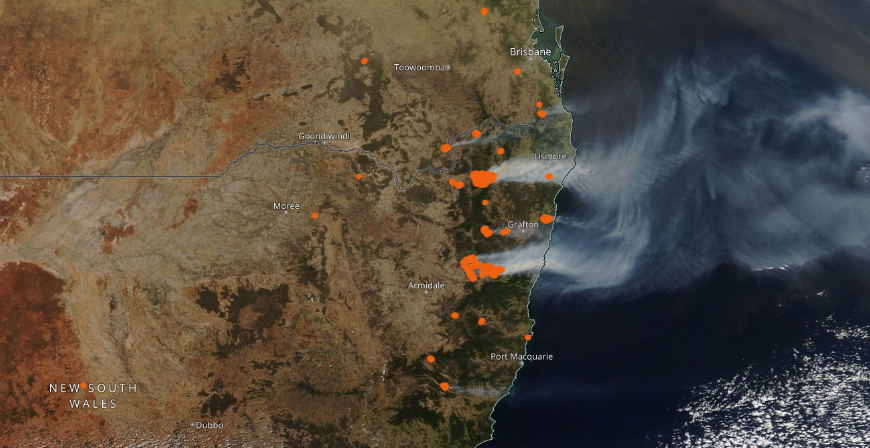
\includegraphics[width=0.9\columnwidth]{images/bushfire.png}
  \newline
  The 2019 Australia bushfires as seen from Aqua's MODIS instrument, annotated with the \textit{Fires and Thermal Anomalies} dataset on NASA's worldview.
\end{frame}

\begin{frame}
  \frametitle{Case Study: Forest fire detection in FIRMS}
  \framesubtitle{Experiment setup}

  \begin{center}
    \includegraphics<1|handout:0>[width=0.8\textwidth]{images/attack_types_1.pdf}%
    \includegraphics<2|handout:0>[width=0.8\textwidth]{images/attack_types_2.pdf}%
    \includegraphics<3|handout:0>[width=0.8\textwidth]{images/attack_types_3.pdf}%
    \includegraphics<4->[width=0.8\textwidth]{images/attack_types_4.pdf}%
  \end{center}

  \footnotetext[1]{NASA source code available with a research account from \url{https://directreadout.sci.gsfc.nasa.gov/}}
  \alt<2->{\footnotetext[2]{Custom tools to pack/unpack CADU frames \url{https://github.com/ssloxford/libcadu}}}{\let\thefootnote\relax\footnotetext{~}}
  \alt<3->{\footnotetext[3]{Custom tools to pack/unpack SPP packets \url{https://github.com/ssloxford/libspp}}}{\let\thefootnote\relax\footnotetext{~}}
  \alt<4->{\footnotetext[4]{Custom tools to modify MODIS sensor readings \url{https://github.com/ssloxford/libgiis}}}{\let\thefootnote\relax\footnotetext{~}}
\end{frame}

\subsection{Attack overview}

% TODO: redo this attack overview re Simon's feedback
\def\footnoterule{\oldfootnoterule}
\begin{frame}
  \frametitle{Attack overview}
  \framesubtitle{Our attack}
  \begin{itemize}[<+->]
    \item Obtain legitimate data from digital archive\footnote<1->[1]{NASA Distributed Active Archive containing MODIS data: \url{https://ladsweb.modaps.eosdis.nasa.gov/archive/}}
   \item Perform security audit on downlink decoder software\footnote<2->[2]{Decoder source code available with an academic account: \url{https://directreadout.sci.gsfc.nasa.gov/}}
   \begin{itemize}
     \item Determine data integrity checks
     \item Identify vulnerabilities where safe input data assumed
   \end{itemize}
    \item Create maliciously crafted data
    \begin{itemize}
      \item Reprocess archived data to add/remove artifacts
      \item Construct payload packet to trigger vulnerability chain
    \end{itemize}
  \end{itemize}
  \note{All the tools used in our attack will be published alongside our paper}
\end{frame}

\subsection{Affecting the derived dataset}

\begin{frame}
  \frametitle{Affecting the derived dataset}
  \framesubtitle{Packet structure}
  \includegraphics<1|handout:0>[width=\textwidth]{images/packet_image_1.pdf}%
  \includegraphics<2|handout:0>[width=\textwidth]{images/packet_image_2.pdf}%
  \includegraphics<3|handout:0>[width=\textwidth]{images/packet_image_3.pdf}%
  \includegraphics<4>[width=\textwidth]{images/packet_image_4.pdf}%
\end{frame}

\begin{frame}
  \frametitle{Affecting the derived dataset}
  \framesubtitle{Attack consequences}
  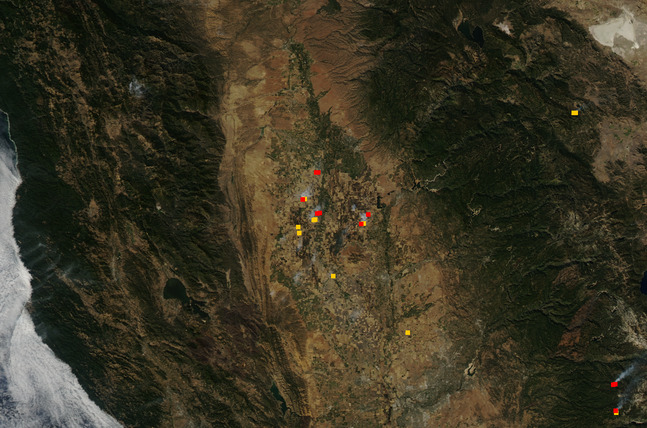
\includegraphics[width=0.7\textwidth]{images/injection/original.jpg}
  \newline
  \centering
  Original image.
\end{frame}

\begin{frame}
  \frametitle{Affecting the derived dataset}
  \framesubtitle{Attack consequences}
  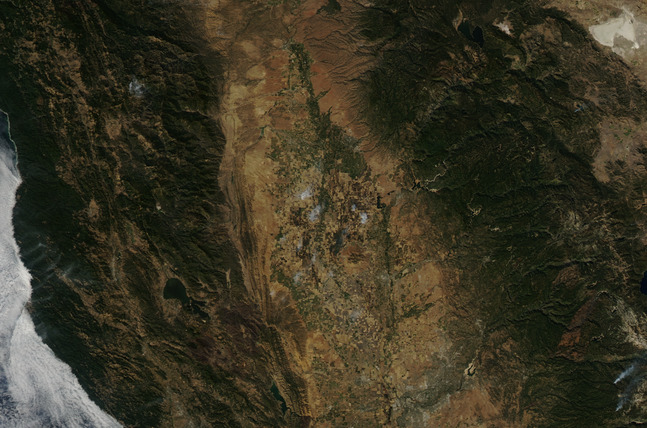
\includegraphics[width=0.7\textwidth]{images/injection/masked_0.jpg}
  \newline
  \centering
  Masking existing fires.
\end{frame}

\begin{frame}
  \frametitle{Affecting the derived dataset}
  \framesubtitle{Attack consequences}
  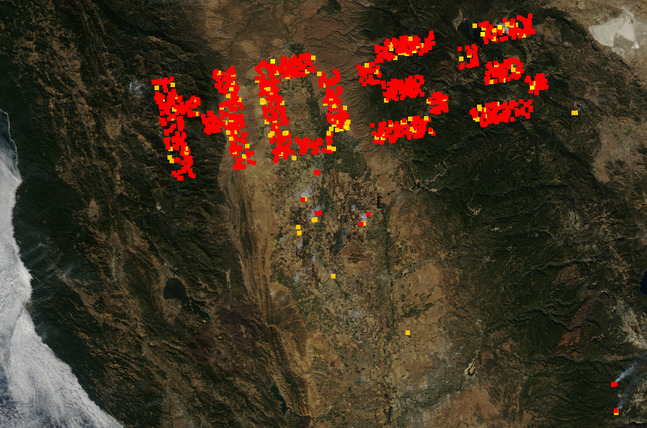
\includegraphics[width=0.7\textwidth]{images/injection/pixels_800_140.jpg}
  \newline
  \centering
  Fine-grained control over fire injection.
\end{frame}

\subsection{Exploiting the decoder}

\begin{frame}
  \frametitle{Exploiting the decoder}
  \framesubtitle{Packet structure}
  \includegraphics<1|handout:0>[width=\textwidth]{images/packet_data_1.pdf}%
  \includegraphics<2|handout:0>[width=\textwidth]{images/packet_data_2.pdf}%
  \includegraphics<3->[width=\textwidth]{images/packet_data_3.pdf}%
\end{frame}

\begin{frame}[fragile]
  \frametitle{Exploiting the decoder}
  \framesubtitle{Attack consequences}
  \begin{lstlisting}[basicstyle=\ttfamily\scriptsize,basewidth=0.6em]
$ printf %1337s  | tr " " "f"  | \
  spppack --type-flag telecommand \
            --sec-hdr-flag 1 \
            --app-id aqua_modis \
  > bad_packet.PDS
  \end{lstlisting}

  \pause
  \begin{lstlisting}[basicstyle=\ttfamily\scriptsize,basewidth=0.6em]
$ cat bad_packet.PDS good_packet_sequence.PDS \
    > ./data/MYD00F.A2015299...001.PDS
  \end{lstlisting}

  \pause
  \begin{lstlisting}[basicstyle=\ttfamily\scriptsize,basewidth=0.6em]
$ ./run_all.sh ./data/
DATA_PATH: /mnt/data
CONTAINER_RUNTIME: docker
  \end{lstlisting}

  \pause
  \begin{lstlisting}[basicstyle=\ttfamily\scriptsize,basewidth=0.6em]
### Processing new PDS:
  MYD00F.A2015299.2110.20152992235.001.PDS
  \end{lstlisting}

  \pause
  \begin{lstlisting}[basicstyle=\ttfamily\scriptsize,basewidth=0.6em]
### Running modisl1db l1a-geo initial processing
<@\textcolor{red}{l0fix\_modis: Unrecoverable error in l0fix\_modis!}@>
  \end{lstlisting}

  \pause
  Further vulnerabilities have been discovered since submission
\end{frame}

\section{Countermeasures}

\def\footnoterule{\only<5->\oldfootnoterule}
\begin{frame}
  \frametitle{Countermeasures}

  Cryptography should be required in future satellites

  \pause
  But existing satellites can't be upgraded
  \newline

  \pause
  Backwards-compatible countermeasures:

  \pause
  \begin{itemize}[<+->]
    \item{Multi-receiver data comparison}
    \item{Timing analysis}\footnote<5->[2]{Jedermann et. al. (2021) ``\textit{Orbit-based Authentication Using TDOA Signatures in Satellite Networks}''}
    \item{Physical-layer fingerprinting}\footnote<6->[3]{Oligeri et. al. (2022) ``\textit{PAST-AI: Physical-Layer Authentication of Satellite Transmitters via Deep Learning}''}
  \end{itemize}
  \newline

  \pause[\thebeamerpauses]

  Existing countermeasures are effective, but aren't viable in all scenarios

  \note{
    \textbf{We discuss the countermeasures in context}

    Multi-receiver data comparison
    \begin{itemize}
      \item Certain systems already have multiple receiver stations
      \item Protects against decoder exploitation
      \item Doesn't require any hardware modifications to the receiver
    \end{itemize}

    Timing analysis
    \begin{itemize}
      \item Triangulating the source effective in other systems such as aircraft
      \item Calculated position can be compared against orbital parameters
      \item Requires accurate clock synchronisation and multiple receivers
    \end{itemize}

    Physical-layer fingerprinting
    \begin{itemize}
      \item Analyse properties of the legitimate/overshadowed signal
      \item Only effective on the downlink
      \item Traditional approaches like analysing signal-to-noise may prove effective
      \item New ML approaches starting to be created (PAST-AI)
    \end{itemize}
  }
\end{frame}

\section{Future work}

\begin{frame}
  \frametitle{Future research directions}
  This work confirms the real-world vulnerability of existing Earth Observing systems

  \pause
  \vspace{0.5cm}
  Future research is required to:

  \pause
  \begin{itemize}[<+->]
    \item Validate this work against real-world receiver hardware
    \item Comprehensively review other vulnerable satellites
    \item Analyze the effectiveness of proposed overshadowing countermeasures
  \end{itemize}

\note{Review of vulnerable satellites: dovetails with other conference work e.g. SAR systems}
\end{frame}

\section{Conclusion}

\begin{frame}
  \frametitle{Conclusion}

  We have...
  \pause
  \begin{itemize}[<+->]
    \item demonstrated viable spoofing attacks against NASA's forest fire detection system.
    \item provided the source code required to manipulate the packet data and structure.
    \item confirmed that only a moderate budget is required to perform these attacks.
    \item identified current countermeasures which significantly increase attack difficulty.
  \end{itemize}
\end{frame}

\begin{frame}
  \frametitle{Thank you for your attention}

  \begin{center}
    \Large
    Any questions?
  \end{center}
  \vspace{0.6cm}

  \begin{center}
    Reach out to me at \\
    \textit{edd.salkield@cs.ox.ac.uk}
  \end{center}
\end{frame}
\end{document}
